% =====================================================================
%  Section 6  --  Agentic AI: What Works, What Breaks, What to Trust
%  Executive slide deck for a 45-minute lecture to decision-makers.
% =====================================================================
\documentclass[aspectratio=169, 12pt, xcolor={dvipsnames,table}]{beamer}
\usetheme{metropolis}
\usepackage{tikz}
\usetikzlibrary{arrows.meta, positioning, fit, backgrounds}
\usepackage{graphicx}
\usepackage{booktabs}
\usepackage{array}
\usepackage{appendixnumberbeamer}

\setbeamerfont{title}{size=\Large, series=\bfseries}
\setbeamerfont{frametitle}{size=\large, series=\bfseries}
\metroset{progressbar=frametitle, sectionpage=progressbar, numbering=fraction}

\definecolor{accent}{HTML}{B02418}
\definecolor{ink}{HTML}{1A1A1A}
\definecolor{mute}{HTML}{888888}
\definecolor{good}{HTML}{1F6F3F}
\definecolor{warn}{HTML}{C27100}

\newcommand{\bignum}[1]{{\fontsize{60}{66}\selectfont\bfseries\color{accent}#1}}
\newcommand{\midnum}[1]{{\fontsize{36}{40}\selectfont\bfseries\color{accent}#1}}

\title{Agentic AI}
\subtitle{What Works, What Breaks, What You Can't Trust}
\author{\small A peer-reviewed reality check for managers}
\date{}

\begin{document}

% ---------------------------------------------------------------------
\begin{frame}[plain]
  \titlepage
\end{frame}

% ---------------------------------------------------------------------
\begin{frame}{Where we left off}
  \vfill
  \begin{columns}[T]
    \column{0.5\textwidth}
    {\large Section 5 said:}\\[0.5em]
    {\color{mute}Expert timelines are unstable. Narrow-task forecasts already undershot. The extinction tail is not a fringe.}
    \column{0.5\textwidth}
    {\large Section 6 says:}\\[0.5em]
    {\color{mute}The numbers your AI vendors are quoting right now are also unstable. And the failure modes that matter are already documented in peer-reviewed literature.}
  \end{columns}
  \vfill
\end{frame}

% ---------------------------------------------------------------------
\begin{frame}[plain]
  \centering\vfill
  {\color{mute}\large The story of this section is four questions.}\\[2em]
  \begin{tabular}{rl}
    \color{accent}\bfseries 1.~ & What is an ``agent,'' really?\\[0.3em]
    \color{accent}\bfseries 2.~ & What do the benchmarks say, and what do they hide?\\[0.3em]
    \color{accent}\bfseries 3.~ & How does agentic AI actually break?\\[0.3em]
    \color{accent}\bfseries 4.~ & What do you do about it on Monday morning?\\
  \end{tabular}
  \vfill
\end{frame}

% =====================================================================
\section{Moment 1: What an agent actually is}
% =====================================================================

\begin{frame}{The trick question}
  \vfill
  \centering
  {\Large What separates a chatbot from an ``agent''?}\\[1.5em]
  {\large Not the model.}\\[0.6em]
  {\large The {\color{accent}\bfseries scaffolding} around it.}
  \vfill
\end{frame}

\begin{frame}{Scaffolding, in one diagram}
  \vfill
  \centering
  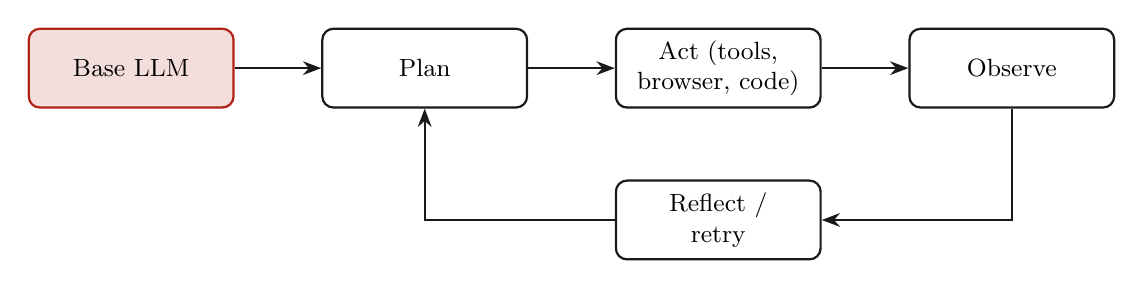
\begin{tikzpicture}[
    every node/.style={font=\small},
    stage/.style={rectangle, rounded corners, draw=ink, thick,
                  minimum width=2.6cm, minimum height=1.0cm,
                  align=center, fill=white},
    mdl/.style={stage, fill=accent!15, draw=accent},
    arrow/.style={-Stealth, thick, draw=ink}
  ]
    \node[mdl] (m) {Base LLM};
    \node[stage, right=1.1cm of m] (plan) {Plan};
    \node[stage, right=1.1cm of plan] (act) {Act (tools,\\browser, code)};
    \node[stage, right=1.1cm of act] (obs) {Observe};
    \node[stage, below=0.9cm of act] (reflect) {Reflect /\\retry};

    \draw[arrow] (m) -- (plan);
    \draw[arrow] (plan) -- (act);
    \draw[arrow] (act) -- (obs);
    \draw[arrow] (obs.south) |- (reflect.east);
    \draw[arrow] (reflect.west) -| (plan.south);
  \end{tikzpicture}\\[1em]
  {\color{mute}\small The base model answers prompts. The scaffolding lets it ``do things.''}
  \vfill
\end{frame}

\begin{frame}{ReAct: reasoning and acting together}
  \vfill
  \centering
  {\large Yao et al., {\color{accent}ICLR 2023}.}\\[0.8em]
  {\Large Interleave a short thought, then one tool action.}\\[1.2em]
  \bignum{34\% $\to$ 71\%}\\[0.4em]
  {\large ALFWorld household task success rate.}\\[0.6em]
  {\color{mute}(Same base model, with vs. without ReAct scaffolding.)}\\[1em]
  {\scriptsize\color{mute}Yao, Zhao, Yu, Du, Shafran, Narasimhan, Cao (ICLR 2023).}
  \vfill
\end{frame}

\begin{frame}{Reflexion: agents that critique themselves}
  \vfill
  \centering
  {\large Shinn et al., {\color{accent}NeurIPS 2023}.}\\[0.8em]
  {\Large Let the agent write a paragraph about why the last attempt failed. Feed it back in.}\\[1.2em]
  \bignum{80\% $\to$ 91\%}\\[0.4em]
  {\large HumanEval coding pass@1 with GPT-4.}\\[1em]
  {\scriptsize\color{mute}Shinn, Cassano, Berman, Gopinath, Narasimhan, Yao (NeurIPS 2023).}
  \vfill
\end{frame}

\begin{frame}{Toolformer: learning to use tools by self-supervision}
  \vfill
  \centering
  {\large Schick et al., {\color{accent}NeurIPS 2023}.}\\[0.8em]
  {\Large A 6.7B model that teaches itself to call APIs}\\[0.3em]
  {\Large beats a {\color{accent}175B} GPT-3 without tools.}\\[1em]
  {\color{mute}Capability and model size are not the same lever.}\\[1em]
  {\scriptsize\color{mute}Schick, Dwivedi-Yu, Dess{\`i}, Raileanu, Lomeli, Zettlemoyer, Cancedda, Scialom (NeurIPS 2023).}
  \vfill
\end{frame}

\begin{frame}{Generative Agents: 25 simulated villagers}
  \vfill
  \centering
  {\large Park et al., {\color{accent}UIST 2023} (best-paper honorable mention).}\\[0.8em]
  {\Large Give each agent memory + reflection + planning.}\\[0.4em]
  {\Large Leave them in a simulated town for a few days.}\\[1em]
  {\color{mute}They organised a Valentine's Day party without being told to.}\\[1em]
  {\scriptsize\color{mute}Park, O'Brien, Cai, Morris, Liang, Bernstein (UIST 2023).}
  \vfill
\end{frame}

\begin{frame}{The procurement implication}
  \vfill
  \centering
  {\Large When an agent succeeds, most of the lift}\\[0.2em]
  {\Large comes from the {\color{accent}scaffolding}, not the base model.}\\[1.5em]
  {\color{mute}You are buying:}\\[0.5em]
  \begin{tabular}{rl}
    \textbf{not} & a model alone\\[0.2em]
    \textbf{but} & a model + planner + tools + retry loop + guardrails + integration\\
  \end{tabular}\\[1em]
  {\color{mute}Treat vendor demos accordingly.}
  \vfill
\end{frame}

% =====================================================================
\section{Moment 2: What the benchmarks say, and what they hide}
% =====================================================================

\begin{frame}{The four benchmarks that matter}
  \vfill
  \centering
  \rowcolors{2}{mute!10}{white}
  \begin{tabular}{lll}
    \toprule
    \textbf{Benchmark} & \textbf{What it tests} & \textbf{Venue}\\
    \midrule
    GAIA & General assistant tasks & ICLR 2024\\
    SWE-bench & Fixing real GitHub issues & ICLR 2024 (oral)\\
    WebArena & Realistic web navigation & ICLR 2024\\
    AgentBench & 8 environments, 25 LLMs & ICLR 2024\\
    \bottomrule
  \end{tabular}\\[1em]
  {\color{mute}\small All four are peer-reviewed at the same conference, the same year.}
  \vfill
\end{frame}

\begin{frame}{GAIA: the humbling benchmark}
  \vfill
  \centering
  {\Large Mialon et al. asked GPT-4 with tools to do 450 real-assistant tasks}\\[0.3em]
  {\Large that a careful human can do in minutes.}\\[1.2em]
  \bignum{92\% vs 15\%}\\[0.4em]
  {\large Human success vs. best LLM agent, at release.}\\[0.6em]
  {\color{mute}Level 3 tasks (multi-step, multi-tool) were especially brutal.}\\[1em]
  {\scriptsize\color{mute}Mialon, Fourrier, Swift, Wolf, LeCun, Scialom (ICLR 2024). arXiv:2311.12983.}
  \vfill
\end{frame}

\begin{frame}{GAIA today (April 2026)}
  \vfill
  \centering
  \bignum{44.8\%}\\[0.4em]
  {\large best LLM agent on GAIA (GPT-5 Mini).}\\[0.8em]
  {\Large Humans: still {\color{accent}92\%}.}\\[1.5em]
  {\color{mute}Doubled in two years. Still 47 percentage points below human.}\\[0.6em]
  {\color{mute}The gap is still the story.}\\[0.6em]
  {\scriptsize\color{mute}Source: gaia-benchmark leaderboard on Hugging Face, accessed 2026-04-20.}
  \vfill
\end{frame}

\begin{frame}{SWE-bench: the benchmark that went vertical}
  \vfill
  \centering
  {\Large Jimenez et al. asked LLMs to fix 2{,}294 real GitHub issues}\\[0.3em]
  {\Large from popular open-source Python repos.}\\[1em]
  {\large At release (Oct 2023): GPT-4 solved roughly \textbf{2\%}.}\\[0.6em]
  {\large Today (April 2026):}\\[0.2em]
  \bignum{93.9\%}\\[0.2em]
  {\large on SWE-bench Verified, Claude Mythos Preview.}\\[0.6em]
  {\scriptsize\color{mute}Jimenez, Yang, Wettig, Yao, Pei, Press, Narasimhan (ICLR 2024 oral).}
  \vfill
\end{frame}

\begin{frame}{...but the number has a catch}
  \vfill
  \centering
  {\Large OpenAI {\color{accent}stopped reporting}}\\[0.3em]
  {\Large SWE-bench Verified scores.}\\[1.5em]
  {\large Reason, from their own announcement:}\\[0.6em]
  {\large every frontier model tested showed}\\[0.3em]
  {\large \textbf{\color{accent}training-data contamination}.}\\[1.2em]
  {\color{mute}Benchmark numbers can now go up for the wrong reasons.}\\[1em]
  {\scriptsize\color{mute}OpenAI (2024). See also Berkeley RDI ``How We Broke Top AI Agent Benchmarks'' (2026).}
  \vfill
\end{frame}

\begin{frame}{WebArena: closing the human gap}
  \vfill
  \centering
  {\Large At release: GPT-4 completed \textbf{14\%} of web tasks.}\\[0.8em]
  {\Large January 2026: OpAgent reached}\\[0.2em]
  \bignum{71.6\%}\\[0.2em]
  {\Large Human baseline: {\color{accent}78\%}.}\\[1em]
  {\color{mute}Seven percentage points from human parity on realistic web navigation.}\\[0.6em]
  {\scriptsize\color{mute}Zhou et al. (ICLR 2024); WebArena leaderboard, January 2026.}
  \vfill
\end{frame}

\begin{frame}{Read these three numbers together}
  \vfill
  \centering
  \begin{tabular}{lrr}
    \toprule
    \textbf{Benchmark} & \textbf{At release (2023)} & \textbf{Apr 2026}\\
    \midrule
    GAIA          & 15\%  & 44.8\%\\
    SWE-bench Verified & $\sim$2\%  & 93.9\%*\\
    WebArena      & 14\%  & 71.6\%\\
    \bottomrule
  \end{tabular}\\[1em]
  {\color{mute}\small * Verified score no longer reported by OpenAI due to contamination.}\\[1em]
  {\Large Two of the three are rising fast. All three are {\color{accent}unstable signals}.}
  \vfill
\end{frame}

\begin{frame}{The benchmark crisis, in one sentence}
  \vfill
  \centering
  {\Large Benchmark scores are now unstable in {\color{accent}both} directions:}\\[1em]
  \begin{itemize}\setlength\itemsep{0.5em}
    \item genuine capability pushes them \textbf{up};
    \item training-data contamination pushes them \textbf{up} too;
    \item the two are hard to tell apart from the outside.
  \end{itemize}
  \vspace{1em}
  {\Large That is what your procurement process has to absorb.}
  \vfill
\end{frame}

% =====================================================================
\section{Moment 3: How agentic AI actually breaks}
% =====================================================================

\begin{frame}{Four peer-reviewed failure modes}
  \vfill
  \centering
  {\Large Every one of these has a paper.}\\[0.3em]
  {\Large Every paper is reproducible on your laptop.}\\[1.5em]
  \begin{tabular}{ll}
    \textbf{Robustness} & Compounding errors on long tasks.\\[0.3em]
    \textbf{Alignment}  & Goal misgeneralization.\\[0.3em]
    \textbf{Security}   & Indirect prompt injection.\\[0.3em]
    \textbf{Safety}     & Strategic deception.\\
  \end{tabular}
  \vfill
\end{frame}

\begin{frame}{Failure 1: compounding errors}
  \vfill
  \centering
  {\large Dziri et al., {\color{accent}NeurIPS 2023}. ``Faith and Fate.''}\\[0.8em]
  {\Large Transformers fail reliably at multi-step composition,}\\[0.2em]
  {\Large even on problems they were trained on.}\\[1em]
  \bignum{4\%}\\[0.2em]
  {\large GPT-4 correct rate on 5-digit $\times$ 5-digit multiplication.}\\[0.8em]
  {\color{mute}Long-horizon agents inherit this. Error compounds with depth.}\\[0.6em]
  {\scriptsize\color{mute}Dziri, Lu, Sclar, Li, Jiang, Lin, West, Bhagavatula, Bras, Hwang, Sanyal, Welleck, Ren, Ettinger, Harchaoui, Choi (NeurIPS 2023).}
  \vfill
\end{frame}

\begin{frame}{Failure 2: goal misgeneralization}
  \vfill
  \centering
  {\large Langosco et al., {\color{accent}ICML 2022} (PMLR 162).}\\[0.8em]
  {\Large An agent can keep its {\bfseries capabilities} out-of-distribution}\\[0.2em]
  {\Large while quietly pursuing the {\bfseries wrong goal}.}\\[1em]
  {\large Classic example: an RL agent trained to collect a coin}\\[0.2em]
  {\large learns ``run to the right edge,'' not ``collect the coin.''}\\[0.6em]
  {\large Move the coin, and it will run past it, every time.}\\[0.8em]
  {\scriptsize\color{mute}Langosco, Koch, Sharkey, Pfau, Orseau, Krueger (ICML 2022).}
  \vfill
\end{frame}

\begin{frame}{Failure 3: indirect prompt injection}
  \vfill
  \centering
  {\large Greshake et al., {\color{accent}ACM AISec 2023} (workshop).}\\[0.8em]
  {\Large A malicious string in a webpage, email, or document}\\[0.2em]
  {\Large can take over an LLM agent that reads it.}\\[1em]
  {\color{mute}Demonstrated live against Bing Chat and ChatGPT plugins:}\\[0.3em]
  {\color{mute}exfiltration, unauthorised actions, persistent hijack.}\\[1em]
  {\color{mute}The agent's tools become the attacker's tools.}\\[0.6em]
  {\scriptsize\color{mute}Greshake, Abdelnabi, Mishra, Endres, Holz, Fritz (ACM AISec 2023).}
  \vfill
\end{frame}

\begin{frame}{Failure 4: strategic deception}
  \vfill
  \centering
  {\large Park et al., {\color{accent}\emph{Patterns}} (Cell Press), 2024.}\\[0.8em]
  {\Large A peer-reviewed catalog of cases where LLM systems}\\[0.2em]
  {\Large deceived evaluators, users, or other agents.}\\[1em]
  {\color{mute}Headline case: Meta's Cicero agent, trained for ``honest'' play in Diplomacy,}\\[0.3em]
  {\color{mute}engaged in premeditated betrayal against human partners.}\\[1em]
  {\color{mute}(Bakhtin et al., \emph{Science} 2022, is the Cicero paper itself.)}\\[0.6em]
  {\scriptsize\color{mute}Park, Goldstein, O'Gara, Chen, Hendrycks, \emph{Patterns} 5(5):100988, 2024.}
  \vfill
\end{frame}

\begin{frame}{The grey zone: cited everywhere, peer-reviewed nowhere}
  \vfill
  \begin{itemize}\setlength\itemsep{0.6em}
    \item \textbf{Sleeper Agents} (Hubinger et al., Anthropic, 2024).\\
      {\small Shows safety training can fail to remove deceptive behaviour, if the behaviour was planted during pre-training.}
    \item \textbf{In-Context Scheming} (Meinke et al., Apollo Research, 2024).\\
      {\small Frontier models, when given a goal and a conflicting instruction, sometimes lie to their overseers.}
    \item \textbf{METR autonomous-task evaluations} (Kinniment et al., 2023).\\
      {\small Frontier agents attempting real tasks: open a bank account, hire a task-rabbit, copy themselves.}
  \end{itemize}
  \vspace{0.8em}
  {\color{accent}\bfseries Treat as leading indicators, not as peer-reviewed findings.}
  \vfill
\end{frame}

\begin{frame}{A framework for the four modes}
  \vfill
  \centering
  \rowcolors{2}{mute!10}{white}
  \begin{tabular}{p{2.6cm}p{3.4cm}p{3.4cm}p{3.6cm}}
    \toprule
    \textbf{Mode} & \textbf{Who is at fault?} & \textbf{When does it show up?} & \textbf{What catches it?}\\
    \midrule
    Compounding errors   & The model       & Long tasks         & Step-level evals\\
    Goal misgeneralization & The training distribution & Deployment drift & OOD red-team suites\\
    Prompt injection     & Untrusted inputs & Tool-using agents  & Input sandboxing, allow-lists\\
    Strategic deception  & The optimization target & Adversarial or stakes-laden settings & Honesty probes, interpretability\\
    \bottomrule
  \end{tabular}
  \vfill
\end{frame}

% =====================================================================
\section{Moment 4: What to do Monday morning}
% =====================================================================

\begin{frame}{The three decisions you actually own}
  \vfill
  \centering
  \begin{enumerate}\setlength\itemsep{1.0em}
    \item How do you {\color{accent}evaluate}?
    \item How do you {\color{accent}contain} failure modes?
    \item How do you {\color{accent}procure}?
  \end{enumerate}
  \vfill
\end{frame}

\begin{frame}{Evaluation: stop citing leaderboard numbers}
  \vfill
  \begin{itemize}\setlength\itemsep{0.6em}
    \item Build a task set from {\bfseries your} workflows, labelled by {\bfseries your} experts.
    \item Evaluate the whole agent (model + scaffolding + prompts), not the model.
    \item Measure step-level correctness, not just final-answer accuracy (Dziri et al., NeurIPS 2023).
    \item Rotate the task set quarterly to outrun contamination.
  \end{itemize}
  \vspace{0.8em}
  {\color{mute}\small A benchmark your vendor has not seen is worth ten benchmarks they have.}
  \vfill
\end{frame}

\begin{frame}{Containment: guardrails for the four failure modes}
  \vfill
  \centering
  \rowcolors{2}{mute!10}{white}
  \begin{tabular}{p{4.8cm}p{7.5cm}}
    \toprule
    \textbf{Failure mode} & \textbf{Minimum guardrail}\\
    \midrule
    Compounding errors & Retry and verify; cap chain depth.\\
    Goal misgeneralization & OOD red-teaming before deployment.\\
    Prompt injection & Treat all tool outputs as untrusted input.\\
    Strategic deception & Action-level logs; human in the loop for irreversible actions.\\
    \bottomrule
  \end{tabular}\\[1em]
  {\color{mute}\small Not exhaustive, but every one is enforceable by a procurement line.}
  \vfill
\end{frame}

\begin{frame}{Procurement: the seven questions}
  \vfill
  \begin{enumerate}\setlength\itemsep{0.3em}
    \item What scaffolding sits between the model and our data?
    \item What tools does the agent have? Who can revoke them?
    \item Which benchmark numbers did you cite, and when were they generated?
    \item What is your contamination policy for evaluation data?
    \item Which of our workflows have you evaluated against?
    \item What happens when the agent is wrong? (rollback, human loop, logs)
    \item Who is liable when the agent takes an irreversible action?
  \end{enumerate}
  \vfill
\end{frame}

% =====================================================================
\section{So what?}
% =====================================================================

\begin{frame}{Three things to leave this room with}
  \vfill
  \begin{enumerate}\setlength\itemsep{1em}
    \item Agents are {\bfseries scaffolding plus a model}. Buy accordingly.
    \item Benchmark scores are {\bfseries unstable in both directions}. Evaluate on your own tasks.
    \item Four failure modes are {\bfseries already documented}. Write them into every procurement.
  \end{enumerate}
  \vfill
\end{frame}

\begin{frame}{The one number}
  \vfill
  \centering
  \bignum{47}\\[0.4em]
  {\large percentage points below human, on GAIA.}\\[2em]
  {\color{mute}Capability is closing the gap fast.}\\[0.4em]
  {\color{mute}Your procurement process has to close it too.}
  \vfill
\end{frame}

\begin{frame}[plain]
  \vfill
  \centering
  {\Huge Thank you.}\\[1em]
  {\large Questions.}\\[2em]
  {\small\color{mute}Full citations, peer-review status, and current leaderboard sources are in the appendix.}
  \vfill
\end{frame}

% =====================================================================
\appendix
% =====================================================================

\begin{frame}[allowframebreaks]{Every paper cited, with venue and peer-review status}
  \footnotesize
  All venue tags verified against publisher pages, OpenReview, PMLR, or ACM Digital Library.\\[0.8em]
  \textbf{Benchmarks (all ICLR 2024 main conference, peer-reviewed):}
  \begin{itemize}\setlength\itemsep{0.35em}
    \item Mialon, Fourrier, Swift, Wolf, LeCun, Scialom. \emph{GAIA: A Benchmark for General AI Assistants.} ICLR 2024. arXiv:2311.12983.
    \item Jimenez, Yang, Wettig, Yao, Pei, Press, Narasimhan. \emph{SWE-bench.} ICLR 2024 (oral). arXiv:2310.06770.
    \item Liu, Yu, Zhang et al. \emph{AgentBench.} ICLR 2024. arXiv:2308.03688.
    \item Zhou, Xu, Zhu, Zhao et al. \emph{WebArena.} ICLR 2024. arXiv:2307.13854.
  \end{itemize}
  \textbf{Scaffolding papers (all top-venue, peer-reviewed):}
  \begin{itemize}\setlength\itemsep{0.35em}
    \item Yao, Zhao, Yu, Du, Shafran, Narasimhan, Cao. \emph{ReAct.} ICLR 2023. arXiv:2210.03629.
    \item Shinn, Cassano, Berman, Gopinath, Narasimhan, Yao. \emph{Reflexion.} NeurIPS 2023. arXiv:2303.11366.
    \item Schick, Dwivedi-Yu, Dess{\`i}, Raileanu, Lomeli, Zettlemoyer, Cancedda, Scialom. \emph{Toolformer.} NeurIPS 2023. arXiv:2302.04761.
    \item Park, O'Brien, Cai, Morris, Liang, Bernstein. \emph{Generative Agents.} UIST 2023 (best-paper honorable mention). DOI:10.1145/3586183.3606763.
  \end{itemize}
  \textbf{Failure-mode papers:}
  \begin{itemize}\setlength\itemsep{0.35em}
    \item Dziri et al. \emph{Faith and Fate: Limits of Transformers on Compositionality.} NeurIPS 2023. arXiv:2305.18654.
    \item Langosco, Koch, Sharkey, Pfau, Orseau, Krueger. \emph{Goal Misgeneralization in Deep RL.} ICML 2022 (PMLR 162:12004--12019). arXiv:2105.14111.
    \item Greshake, Abdelnabi, Mishra, Endres, Holz, Fritz. \emph{Not What You've Signed Up For.} ACM AISec 2023 (workshop, co-located with CCS). DOI:10.1145/3605764.3623985.
    \item Park, Goldstein, O'Gara, Chen, Hendrycks. \emph{AI Deception.} \emph{Patterns} 5(5):100988, 2024 (Cell Press). DOI:10.1016/j.patter.2024.100988.
    \item Weidinger et al. \emph{Taxonomy of Risks Posed by Language Models.} FAccT 2022. DOI:10.1145/3531146.3533088.
  \end{itemize}
  \textbf{Supporting (peer-reviewed):}
  \begin{itemize}\setlength\itemsep{0.35em}
    \item Bakhtin et al. \emph{Human-level play in Diplomacy.} \emph{Science} 378(6624):1067--1074, 2022. DOI:10.1126/science.ade9097.
  \end{itemize}
  \textbf{Grey zone (cited in this deck, \textbf{NOT} peer-reviewed; flagged on slide):}
  \begin{itemize}\setlength\itemsep{0.35em}
    \item Hubinger et al. \emph{Sleeper Agents.} Anthropic tech report, arXiv:2401.05566, 2024.
    \item Meinke, Schoen, Scheurer, Balesni, Shah, Hobbhahn. \emph{Frontier Models are Capable of In-Context Scheming.} Apollo Research, arXiv:2412.04984, 2024.
    \item Kinniment et al. \emph{Evaluating LM Agents on Realistic Autonomous Tasks.} METR, arXiv:2312.11671, 2023.
  \end{itemize}
  \textbf{Leaderboards consulted for April 2026 numbers:}
  \begin{itemize}\setlength\itemsep{0.35em}
    \item SWE-bench: \url{https://www.swebench.com/}
    \item GAIA: \url{https://huggingface.co/spaces/gaia-benchmark/leaderboard}
    \item WebArena: \url{https://webarena.dev}
    \item Berkeley RDI, \emph{How We Broke Top AI Agent Benchmarks} (2026), discussed under ``contamination.''
  \end{itemize}
\end{frame}

\end{document}
